\documentclass[a4paper]{article}
\usepackage[a4paper,margin=1in,includefoot]{geometry}
\usepackage[utf8]{inputenc}
\usepackage{hyperref}
\usepackage{float}
\usepackage{graphicx}
\usepackage{caption}
\usepackage{subcaption}
\usepackage{xcolor}
\usepackage{amsmath}
\usepackage{siunitx}
\usepackage{tabularx}
\usepackage{booktabs}
\usepackage{enumitem}
\usepackage[us,nodayofweek]{datetime}
\usepackage[style=alphabetic,maxbibnames=99,giveninits]{biblatex}
\captionsetup{font=footnotesize}
\addbibresource{references.bib}
\graphicspath{{./images/}}
\newcommand*{\img}[1]{%
    \raisebox{-.25\baselineskip}{%
        \includegraphics[
        height=\baselineskip,
        width=\baselineskip,
        keepaspectratio,
        ]{#1}%
    }%
}

\title{Super Mario World AI}
\author{Siebren Cosijn}
\newdate{date}{31}{08}{2022}
\date{\displaydate{date}}
\begin{document}
\maketitle

\section{Introduction} \label{s:introduction}
This graduate work is based on the popular game Super Mario World, developed by Nintendo for the SNES\footnote{Super Nintendo Entertainment System}.
The game consists of many different levels, during which the objective is to reach the ``goalpost'' to advance to the next level before the timer runs out.
To achieve this Mario will have to jump over and on top of platforms, avoid obstacles, and defeat enemies.
\begin{figure}[htbp]
    \centering
    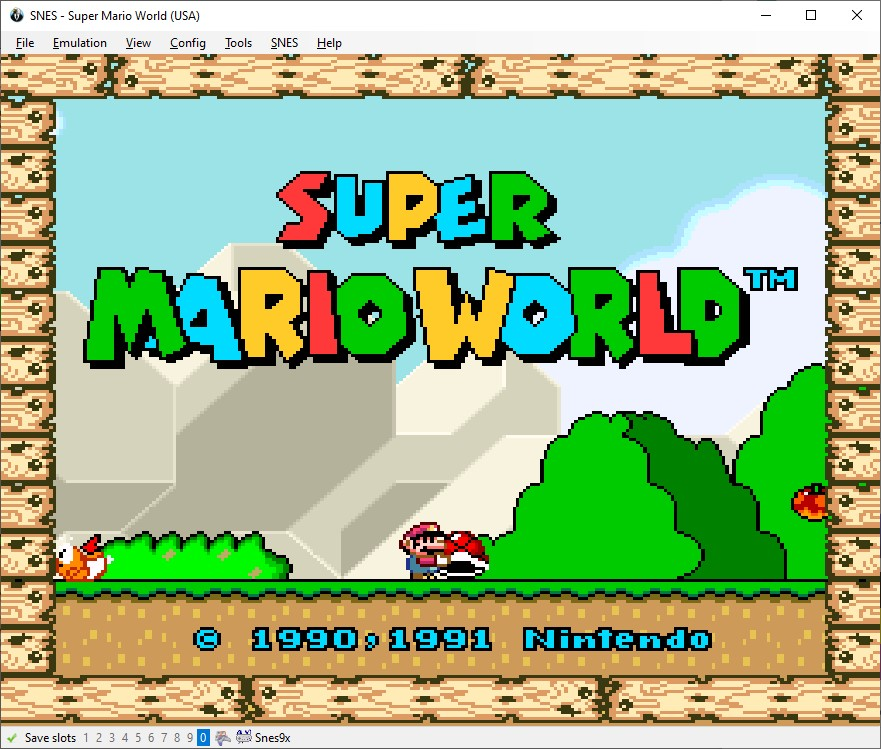
\includegraphics[width=.6\textwidth]{start-screen}
    \caption{Screenshot of the Super Mario World start screen.}
    \label{fig:smw}
\end{figure}

The goal of this work is to teach an AI how to play the game using reinforcement learning.
We train an agent on some of the more basic levels and observe how it learns to deal with the various obstacles presented by the game.
Afterwards we evaluate how the agent performs on those levels and see if it can successfully complete them.
For this task we use OpenAI Gym\footnote{\url{https://github.com/openai/gym}} (a library for developing and comparing reinforcement learning algorithms) and Gym Retro\footnote{\url{https://github.com/openai/retro}} (additional game integrations for Gym, including Super Mario World).

\section{Reinforcement Learning} \label{s:reinforcement-learning}
Reinforcement learning (RL) is an area of machine learning which studies how intelligent agents learn to take actions in an environment by trial and error.
An agent is not told which actions to take, but must explore for itself which actions result in the highest reward.
The general idea behind RL is that rewarding good behavior or penalizing bad behavior makes the agent more or less likely to repeat this behavior in the future.
How the agent interacts with its environment is shown in the agent-environment loop in Figure \ref{fig:loop}.
\begin{figure}[htbp]
    \centering
    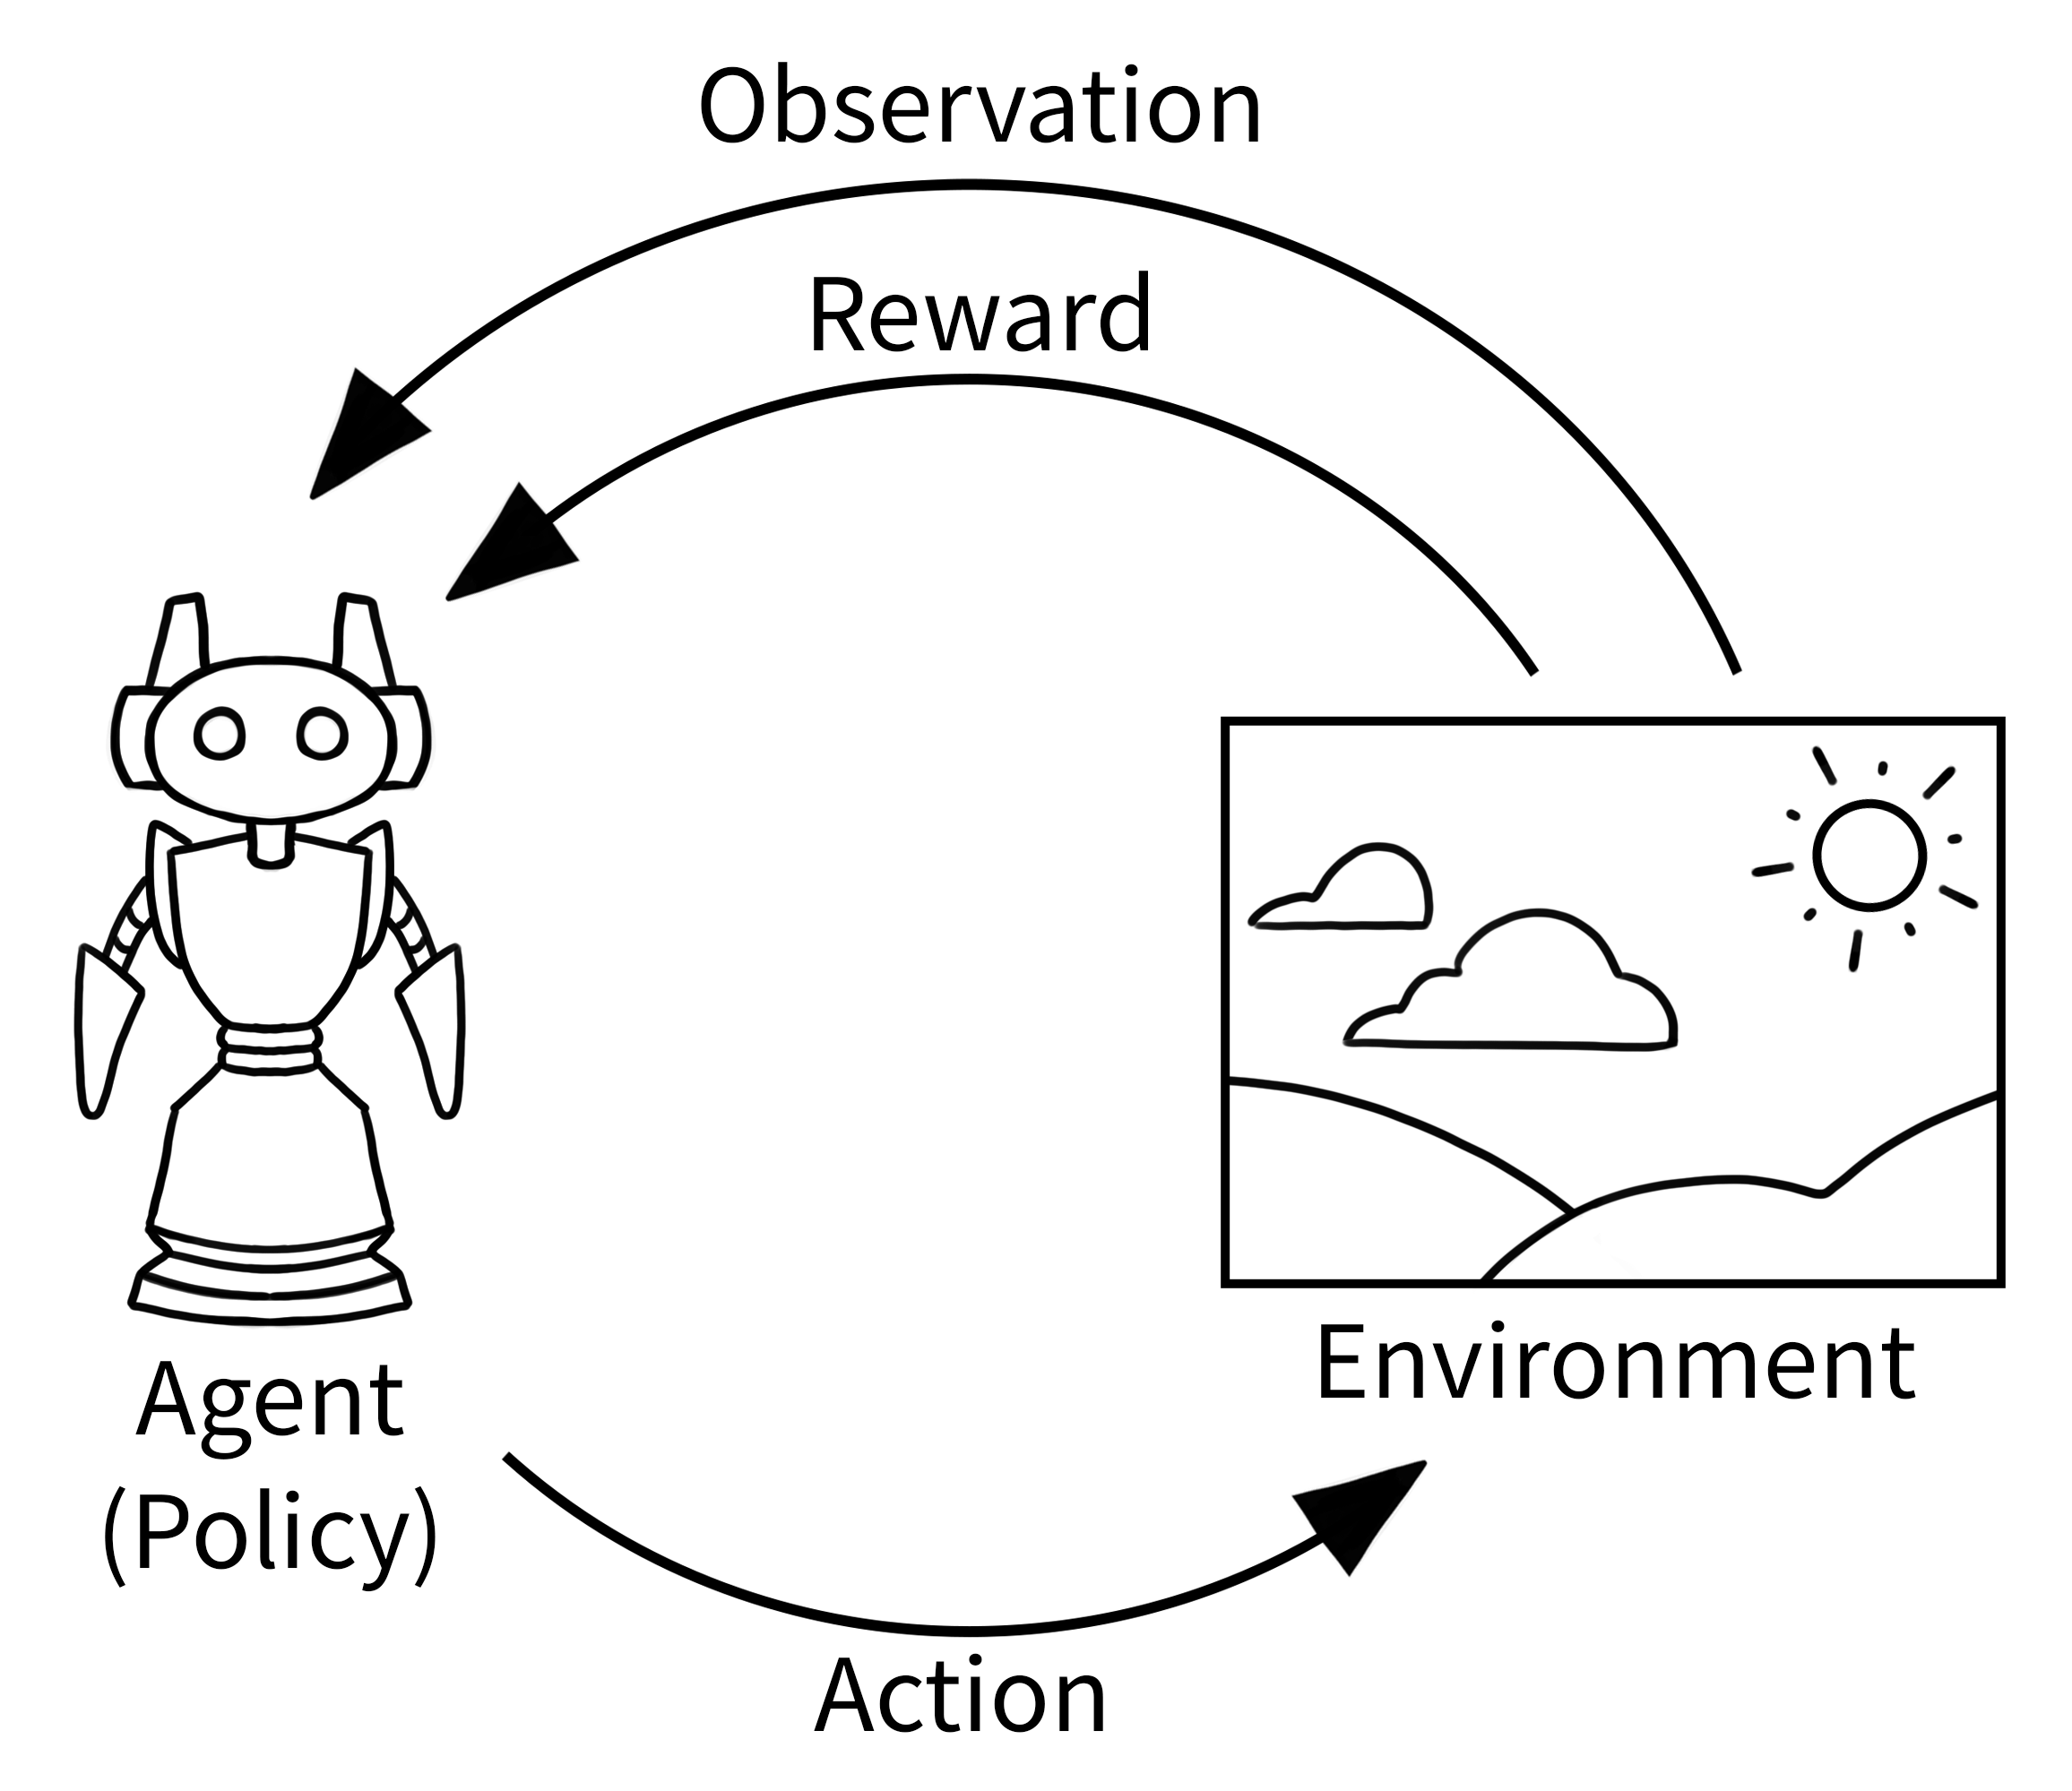
\includegraphics[width=.6\textwidth]{AE_loop}
    \caption{The agent-environment interaction loop. Image source: \url{https://www.gymlibrary.dev}.}
    \label{fig:loop}
\end{figure}

The agent is trained in episodes which consist of a number of steps.
At each step, the agent receives the current observation and reward.
It then chooses an action to perform on the environment.
The action changes the state of the environment, and the environment returns a new observation and a reward based on how the action influenced the state.
Each component of the agent-environment interaction is described in more detail below.
\begin{description}[leftmargin=0cm]
    \item[Agent.]
    The decision maker of the process.
    How the agent chooses its actions is decided by a policy that tries to maximize the some form of cumulative reward.
    In our case the agent controls Mario and decides which actions he will take.
    \item[Action.]
    Agents interact with their environment through actions.
    In this game, an action is a combination of button presses.
    The set of all valid actions in an environment is called the \emph{action space}.
    \item[Environment.]
    World that the agent lives in (level of the game).
    The environment is represented by states, which are complete descriptions of the world.
    \item[Observation.]
    Part of the state that the agent is able to see (i.e., its immediate surroundings).
    Observations are, in this case, ``frames'' of the game.
    A frame is an image of the game; a raster of pixels of the form height\texttimes{}width\texttimes{}channel.
    The \emph{observation space} defines the structure and legitimate values an observation can take.
    \item[Reward.]
    A numeric value that describes how good (or bad) the result of an action is on the state of the environment.
    The value is determined by the reward function (more on rewards in Section \ref{s:reward}).
\end{description}

\section{Preprocessing} \label{s:preprocessing}
Before we can train our agent a number of preprocessing steps are necessary.
This includes a transformation of both the action and observation space.
Most of these steps are based on papers discussing the Arcade Learning Environment (ALE) \cite{bellemare2013arcade,machado2018revisiting}.
The ALE is a framework that allows people to develop AI agents for Atari\footnote{Atari 2600, originally known as Atari VCS (Video Computer System)} games and is commonly used to benchmark reinforcement learning algorithms.
Even though the ALE was created for Atari games, most of the preprocessing steps used are also applicable to the SNES (and Super Mario World).

\subsection{Action Space}
By default, the Gym Retro environment for Super Mario World uses a MultiBinary\footnote{\url{https://www.gymlibrary.dev/content/spaces/\#multibinary}} space with 12 elements (buttons).
Each action contains a value for every button in the action space where 0 (not pressed) or 1 (pressed). This results in $2^{12}=4096$ possible combinations.
Sticking to the default MultiBinary action space leads to three issues:
\begin{itemize}
    \item \textbf{Large action space.}
        Exploration in RL relies on some form of random sampling.
        If the action space is large, it will take longer for the agent to find good actions during exploration.
    \item \textbf{Invalid combinations.}
        Some combinations of buttons cannot be pressed at the same time (e.g. left and right arrows).
    \item \textbf{Irrelevant buttons.} Some buttons are only used to control the game menu or pause the game and have no effect on the actual gameplay.
\end{itemize}
To solve these problems we take a look at the SNES controller in Figure \ref{fig:snes-controller}.
The game was designed to be played on this controller, so the buttons used in Gym Retro correspond to the buttons on this controller.
Select, start, and the buttons on the back of the controller are not relevant for our agent.
The remaining buttons can be split into two clusters, arrow keys and special keys.
For each cluster, only one button can be pressed at any given time.
This translates to a MultiDiscrete\footnote{\url{https://www.gymlibrary.dev/content/spaces/\#multidiscrete}} action space, which is the cartesian product of (in this case two) discrete spaces.
The actions of both discrete spaces are described below.
In this game the \img{SuperNintendo-Button-X} and \img{SuperNintendo-Button-Y} keys serve the same function, so we only need to include one of them.
Not pressing a button is also a valid action.
\begin{itemize}
    \item \textbf{Arrow keys.} none, left (\img{SuperNintendo-Dpad-Left}), right (\img{SuperNintendo-Dpad-Right}), up (\img{SuperNintendo-Dpad-Up}), down (\img{SuperNintendo-Dpad-Down})
    \item \textbf{Special keys.} none, spin (\img{SuperNintendo-Button-A}), jump (\img{SuperNintendo-Button-B}), run/throw (\img{SuperNintendo-Button-X})
\end{itemize}
\begin{figure}[htbp]
    \centering
    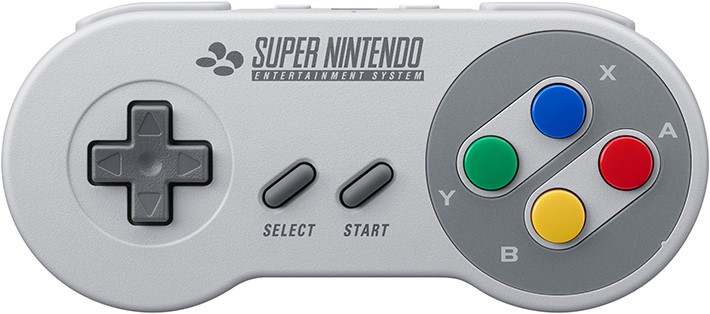
\includegraphics[width=.7\textwidth]{snes-controller}
    \caption{SNES controller.}
    \label{fig:snes-controller}
\end{figure}
The resulting MultiDiscrete action space contains $5\cdot4 = 20$ different actions.
So we have reduced the action space by a significant amount while maintaining the necessary actions to play the game.

\subsection{Observation Space}
\subsubsection{Transform observation}
To reduce the memory requirement, each observation is resized from 256\texttimes{}224 to 84\texttimes{}84 pixels.
The color is also converted from RGB to grayscale.
Figure \ref{fig:transformation} shows the result of this transformation.
Lowering the memory requirement significantly reduces the training time of the agent.
\begin{figure}[htbp]
    \centering
    \begin{subfigure}{.5\textwidth}
        \centering
        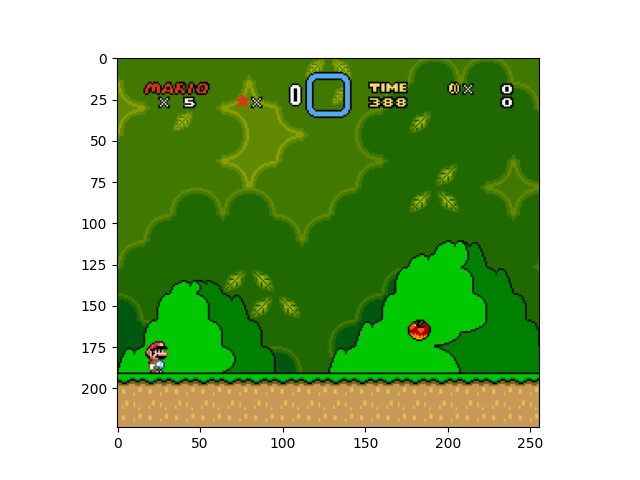
\includegraphics[height=6.35cm]{original}
        \caption{Original}
        \label{fig:transformation:sub1}
    \end{subfigure}%
    \begin{subfigure}{.5\textwidth}
        \centering
        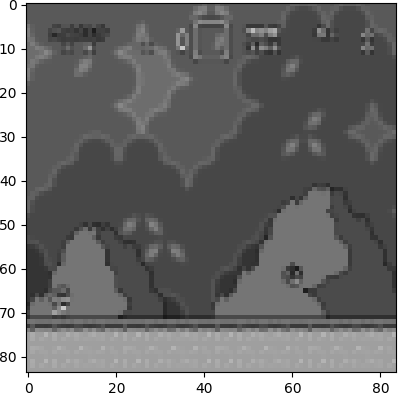
\includegraphics[height=6.35cm]{grayscale}
        \caption{Transformed}
        \label{fig:transformation:sub2}
    \end{subfigure}
    \caption{Transforming the observation. Resized to 84\texttimes{}84 pixels and converted to grayscale.}
    \label{fig:transformation}
\end{figure}

\subsubsection{Skip frames}
Super Mario World runs at 60 FPS (frames per second), which means there is little change in the game from frame to frame.
As a result, there is no need to input a new action for each frame.
Having the agent decide on a new action every few frames instead of every single frame speeds up the execution, allowing it to play more episodes during training.
To create this effect of ``skipping'' frames each action is repeated over four frames and only the last frame is returned as observation, together with the sum of the accumulated rewards.

\subsubsection{Stack frames}
The agent is trained on pixels, so each observation can be seen as some sort of screenshot of the game state.
By using a single frame, the agent cannot perceive the direction or velocity of movement (Is Mario going up or down? How fast is Mario moving?).
To solve this we ``stack'' four subsequent observations and use the result as input for the agent.
Each observation is concatenated with the previous three most recent observations.
In Figure \ref{fig:stack} we can see based on a stack of four observations that Mario is jumping to the right.
\begin{figure}[htbp]
    \centering
    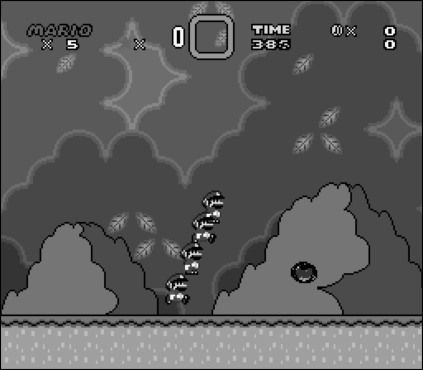
\includegraphics[height=6cm]{stacked}
    \caption{A frame stack of four subsequent observations.}
    \label{fig:stack}
\end{figure}

\subsection{Other}
\subsubsection{Episodic Life}
In Gym environments, the current episode ends when the ``done'' signal is received.
However, in this game the player starts with five lives, so this signal is only sent once the life counter reaches zero.
Every time Mario dies the game exits the current level and returns to the level selection menu.
Since no signal has been sent, the agent does not understand it is no longer in the intended level, and as a result can get stuck in the menu or even enter another level by accident.
To avoid this we want to terminate the episode after a single life is lost.
Ending the episode after a life is lost also creates a positive side effect; the longer the episode continues, the more rewards the agent can gain, so the agent learns to avoid death without explicitly defining a penalty for losing a life.

\subsubsection{Sticky Actions}
Super Mario World is largely deterministic. 
Most enemies and other moving objects will always appear in the same location at the same timestamp of a level.
We want the agent to learn to make good decisions in various game scenarios, not just memorize one action sequence in a single level, so we need to introduce some form of stochasticity.
With ``sticky actions'' \cite{machado2018revisiting} each time the agent chooses a new action there is a 25\% chance it will repeat the previous action instead.
This makes it so the agent is never sure where it will end up at any given time, and forces it to act accordingly.

\section{Reward} \label{s:reward}
The goal of an agent in reinforcement learning is to maximize its cumulative reward.
After each step the agent receives a reward from the environment, which describes how good (or bad) the action taken during this step was.
The value of this reward is determined by the reward function.
A well designed reward function is important in order for the agent to achieve the desired behavior.

Gym Retro's default rewards are most often tied to the game score.
In Super Mario World the player gains points by collecting coins or defeating enemies.
However, the goal of a human player is usually beating the game by completing all the different levels, not maximizing the score.
When trained using the score as reward, the agent will find some unintended way to maximize its score (defeating the same enemy over and over, for example) without ever finishing a level.
An alternative reward is needed if we want the agent to act similar to human players.

In theory you could design a reward function that gives $+1$ for completing a level of the game.
This reward is not practical though, because it is too ``sparse''.
The duration of a single episode is limited to several thousand steps due to the timer present in the game.
It is very unlikely the agent will reach the end of a level by taking random actions before the timer expires, so it might never see a positive reward.
The agent cannot learn which actions are good with such a restrictive reward.
So we are looking for some reward that is easier to obtain but should still result in completing a level if maximized.

Mario starts each level on the left side and the flag which indicates the end of that level is always on the right side.
We can reward the agent for moving right by comparing Mario's horizontal position (x-value) before and after each step.
Subtracting the x-value $x_{t}$ at step $t$ with that of the previous step $x_{t-1}$ can result in the following three scenarios.
\begin{eqnarray*}
    x_{t} - x_{t-1} > 0&\iff&\text{Mario is moving to the right}\\
    x_{t} - x_{t-1} = 0&\iff&\text{Mario is standing in place}\\
    x_{t} - x_{t-1} < 0&\iff&\text{Mario is moving to the left}
\end{eqnarray*}
The magnitude of the reward is determined by how much Mario moved in a single step.
Moving faster will result in a larger reward (or penalty in case of moving left).

There is one more simple improvement we can make.
By applying a small penalty ($-1$) on each step we incentivize the agent to try to complete the level as fast as possible.
Combining both gives us the reward $r_{t}$ at each step $t$.
\[r_{t} = x_{t} - x_{t-1} - 1\]


\section{Algorithm} \label{s:algorithm}
With the preprocessing and reward design completed, only the choice of algorithm remains before we can start training.
Reinforcement learning algorithms can be divided into two branches: \emph{Model-Based RL} and \emph{Model-Free RL}.
In model-based RL the agent uses a model (a function which predicts how the environment will react to actions) to make decisions.
The model can either be known beforehand (not the case here) or learned through interaction with the environment.
The main advantage of model-based algorithms is that they are sample efficient; they learn the most out of each experience.
By contrast, model-free algorithms sample purely from experience instead of using predictions of the next state.
In general, model-free methods are computationally cheaper than having to learn a model of the environment, with the trade-off of being less sample efficient.
In the case of Super Mario World we opt for a model-free approach because the policy is easier to learn than the model and interaction with the environment is fast.

Model-free RL can be further divided into two main approaches: \emph{Q-Learning} and \emph{Policy Optimization}.
Q-learning methods try to learn or approximate the optimal action-value function.
This means they learn the value of state-action pairs and take the action that leads to the most valuable state.
Finding the optimal action-value function will also result in the optimal policy.
Q-learning methods (with function approximation) tend to be less stable and are not guaranteed to converge.
However, when they work they are more sample efficient than policy optimization techniques, because they can reuse old data more effectively.
Policy optimization methods try to directly optimize the policy.
The probabilities of actions are modeled using a neural network.
Through interaction of the agent with the environment the parameters of the network are tweaked, so that good actions are more likely to be sampled in the future.
The main advantage of policy optimization methods is that they are stable and reliable.

Proximal Policy Optimization (PPO) \cite{schulman2017proximal} is a state-of-the-art policy optimization algorithm.
PPO updates policies by taking the largest possible step to improve performance, without stepping so far that it accidentally causes the performance to collapse.
It achieves this by introducing a new hyperparameter, $\epsilon$, which defines the clipping range.
The use of this parameter restricts the probability ratio (a measure of the difference between old and new policy) to the interval $[1-\epsilon,1+\epsilon]$.
This clipping puts a constraint on how far the new policy can be removed from the old to avoid destructively large policy updates.
Some advantages of PPO are: stable and reliable, easy to tune (not too reliant on finding the best hyperparameters), easy to parallelize by collecting experience from multiple copies of an environment and processing it in batches;
which makes it a good choice for this project.
We use the implementation of PPO from the Stable Baselines3 library\footnote{\url{https://github.com/DLR-RM/stable-baselines3}}.

\subsection{Hyperparameters}
The following hyperparameters for PPO were used to train the agent.
Unmentioned hyperparameters use the default value defined in the Stable Baselines library.
\begin{table}[htbp]
\centering
\begin{tabularx}{\linewidth}{llX}
\toprule
Hyperparameter & Value & Description \tabularnewline
\midrule
learning\_rate & \num{1e-4} & Learning rate of the Adam optimizer. \tabularnewline
n\_steps & 512 & Number of steps of experience to collect for each environment before a policy update. Buffer size is equal to n\_steps $\times$ n\_envs. \tabularnewline
n\_envs & 8 & Number of environment copies running in parallel. \tabularnewline
batch\_size & 512 & Minibatch size. How many experiences to use for each gradient update. Must be a fraction of buffer size. \tabularnewline
n\_epochs & 2 & Number of epochs to run for each minibatch. Less epochs will ensure more stable updates, at the cost of slower learning. \tabularnewline
clip\_range & 0.1 & Clipping parameter ($\epsilon$). A larger clipping range means the new policy can diverge more from the old policy. Small values will result in more stable updates, but will also slow the learning process. \tabularnewline
ent\_coef & 0.001 & Entropy coefficient. Prevents the policy from converging too quickly. Larger values keep the policy random for longer, resulting in more exploration. \tabularnewline
\bottomrule
\end{tabularx}
\caption{PPO hyperparameters used for training the Super Mario World agent.}
\label{table:hyperparams}
\end{table}

\section{Training \& Results} \label{s:training-results}
\subsection{Model I}
In this model the agent was trained for 25 million timesteps on the first level of the game, ``Yoshi's Island 1''.
Figure \ref{fig:result1} shows the mean episode length and reward during training.
\begin{figure}[htbp]
    \centering
    \begin{subfigure}{.5\textwidth}
        \centering
        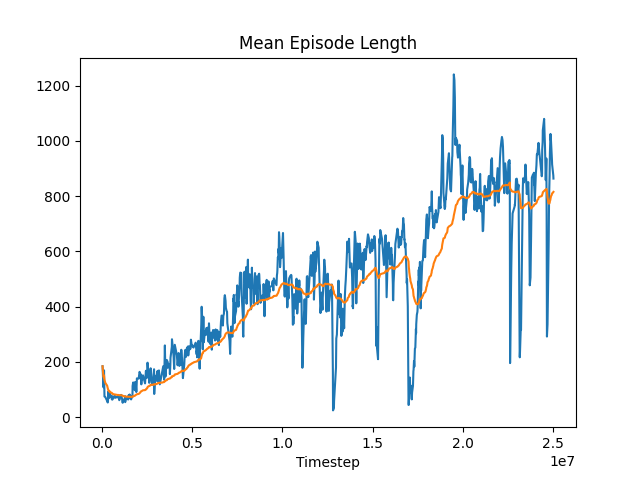
\includegraphics[width=\textwidth]{PPO_YoshiIsland1_len}
        \label{fig:result1:sub1}
    \end{subfigure}%
    \begin{subfigure}{.5\textwidth}
        \centering
        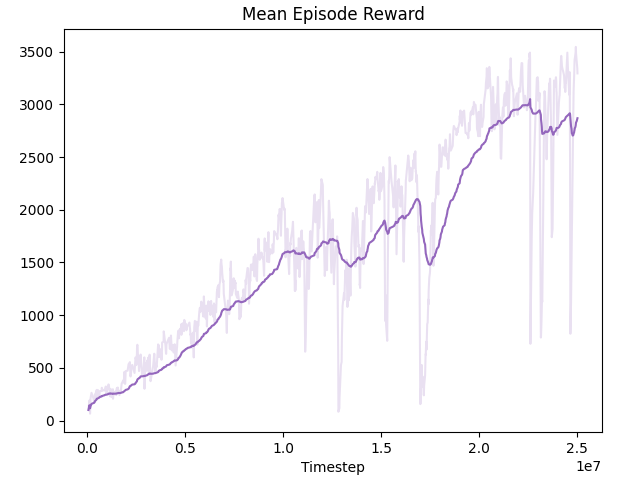
\includegraphics[width=\textwidth]{PPO_YoshiIsland1_rew}
        \label{fig:result1:sub2}
    \end{subfigure}
    \caption{Results of training on the level YoshiIsland1 for 25M timesteps.}
    \label{fig:result1}
\end{figure}

\noindent Video of the agent playing the first level: \href{https://user-images.githubusercontent.com/17729237/187476061-c6c80b38-291d-4d32-b37c-6c923a414eeb.mp4}{\color{blue}{Yoshi's Island 1}}

\subsection{Model II}
\begin{figure}[htbp]
    \centering
    \begin{subfigure}{.5\textwidth}
        \centering
        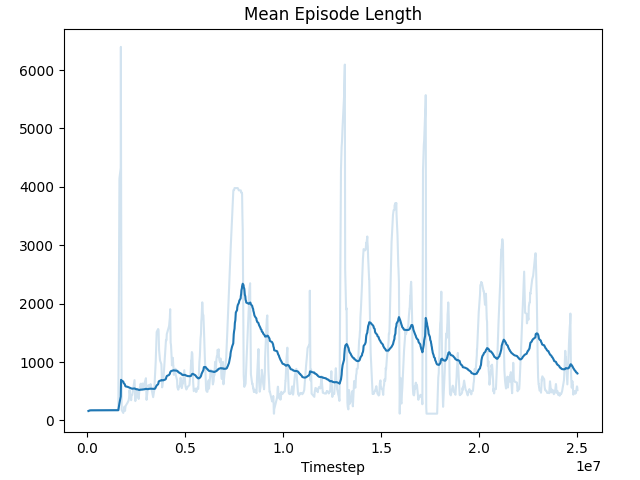
\includegraphics[width=\textwidth]{PPO_YoshiIsland2_len}
        \label{fig:result2:sub1}
    \end{subfigure}%
    \begin{subfigure}{.5\textwidth}
        \centering
        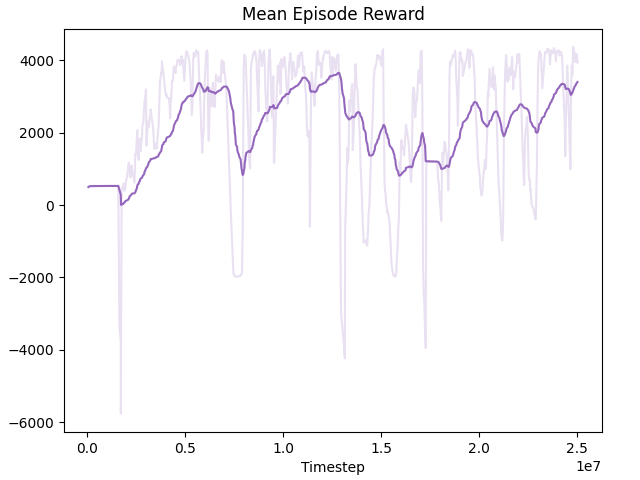
\includegraphics[width=\textwidth]{PPO_YoshiIsland2_rew}
        \label{fig:result2:sub2}
    \end{subfigure}
    \caption{Results of training on the level YoshiIsland2 for 25M timesteps.}
    \label{fig:result2}
\end{figure}
\noindent Video of the agent playing the second level: \href{https://user-images.githubusercontent.com/17729237/187476212-73ea3e18-d42b-4225-8ae2-7bb87132dab3.mp4}{\color{blue}{Yoshi's Island 2}}

\printbibliography
\end{document}